%% chapter1.tex 
%
\chapter{Introduction}
Single image super resolution using deep learning is one of the key area of research in recent times. Conventionally the resolution of images was increased using various interpolation techniques like bicubic interpolation, Nearest neighbour interpolation, bilinear interpolation etc. However, these techniques are not very efficient and looses minute features from images. These minute features are of great importance in medical images. Hence Deep learning based approaches explored to overcome this problem. Deep learning algorithms in Wireless Capsule Endoscopy (WCE) image analysis are a promising research area to overcome the pitfalls presented in the hand-crafted feature selection method. Medical Images contains a lot of complex data, which is easily missed while dealing with hand crafted features.

\section{Capsule Endoscopy}
Endoscopy is a common imaging procedure that may be utilised for diagnostic as well as minimally invasive surgical treatment. Video Capsule Endoscopy (VCE) is a ground-breaking imaging technology that allows for unparalleled direct vision of the gastrointestinal tract with little patient discomfort. A normal colon VCE test generates around 8 hours of RGB video data. Wireless Capsule Endoscopy (WCE) is a non-invasive procedure for detecting irregularities in the Gastro intestinal tract of humans. It consists of an optical dome, illuminator, imaging sensor, battery, and RF transmitter in a capsule-shaped item with a length of 26 mm and a diameter of 11 mm. During the examination, the patient swallows the WCE and then slides it slowly down the small intestine, taking photos of the whole gastro intestinal tract while doing so. As shown in Fig.~\ref{fig:label1.1} Finally, these images are transferred wirelessly to a data-recording device so that doctors can study the photos later for diagnosis. While moving through the gastro intestinal tract, an average of 50k to 60k images are taken. It is a time-consuming and arduous operation for the medico to verify all 60k images in order to find any abnormalities in the gastro intestinal tract. 

\begin{figure}[h]
    \centering
    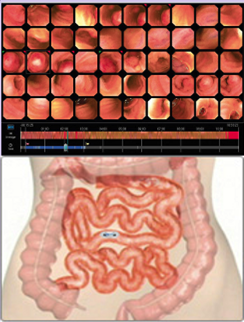
\includegraphics[totalheight=2.5in]{Chapter1/Fig4.png}
    \caption[The capsule movement in the gastro-intestinal track and also provides theglimpse of images captured by the capsule camera during its journey ingastrointestinal track]{The capsule movement in the gastro-intestinal track and also provides theglimpse of images captured by the capsule camera during its journey ingastro-intestinal track.\cite{Capsule}}
    \label{fig:label1.1}
\end{figure}

\begin{figure}[h]
    \centering
    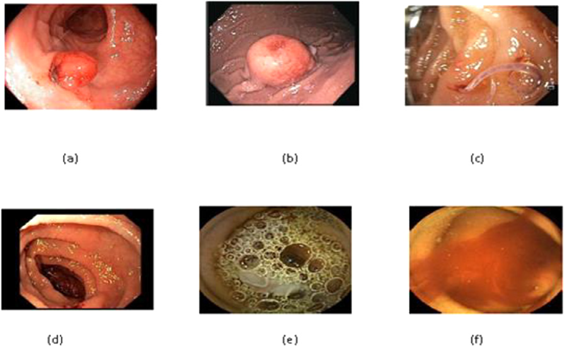
\includegraphics[totalheight=2.0in]{Chapter1/Fig5.png}
    \caption[(a) Polyp, (b) Tumour (c) Hookworm (d) Celiac (e) Bubbles (f) Bleeding]{(a) Polyp, (b) Tumour (c) Hookworm (d) Celiac (e) Bubbles (f) Bleeding. \cite{Capsule}}
    \label{fig:label1.2}
\end{figure}
The small bowel is located in the middle of the gastrointestinal (GI) tract, between the stomach and the large intestine. It is three to four metres long and has a surface area of roughly 30 \(m^2\) ,including the villi's surface area, and plays an important role in nutrient absorption. As a result, small bowel problems can cause significant development retardation in children as well as nutritional deficiencies in both children and adults. Chronic illnesses such as Crohn's disease, celiac disease, and angiectasis, as well as malignant diseases such as lymphoma and adenocarcinoma, can damage this organ.
%\newline

These illnesses can pose a significant health risk to individuals and society, and diagnosing and treating them often necessitates a comprehensive inspection of the lumen. The small intestine, on the other hand, is less accessible for inspection by flexible endoscopes frequently employed for the upper GI tract and the large bowel due to its anatomical position. VCE has been utilised as a supplementary diagnostic for patients with GI bleeding since the early 2000s. A VCE is a tiny capsule that houses a wide-angle camera, as well as light sources, batteries, and other electronics. The patient eats the capsule, which records video as it travels through the GI tract passively. The glimpse of images taken by capsule is provided in Fig.~\ref{fig:label1.2}
\section{Image Super Resolution}
The process of converting one or more low-resolution observations of the same scene into high-resolution photographs is known as Super-Resolution (SR). The SR can be divided into Single Image Super Resolution (SISR) and Multi-Image Super-Resolution (MISR) depending on the quantity of input LR images. SISR is far more well-liked than MISR due to its great effectiveness. High perceptual quality HR images are employed extensively in a variety of fields, including security imaging, satellite imaging, and medical imaging because they contain more useful details. In the typical SISR framework, as depicted in Fig.~\ref{fig:label1.3}. Eq.~\ref{eq:1.1} shows the LR image $y$ is degraded due to blur, downsampling and noise effect.  
\begin{equation} \label{eq:1.1}
y=(x \otimes k) \downarrow_{s}+n
\end{equation}
where, x $\otimes{}$ k is the convolution between the blurry kernel $k$ and the unknown HR image $x$, $\downarrow_{s}$ represents the downsampling operator with scale factor $s$, and $n$ is the independent noise term. Solving equation (~\ref{eq:1.1}) is an extraordinarily ill-posed problem due to the fact that a single LR input may correlate to several HR solutions. Interpolation-based approaches, reconstruction-based methods, and learning-based methods make up the majority of the prevalent SISR algorithms in recent times \cite{DLSR}.
\begin{figure}[h]
    \centering
    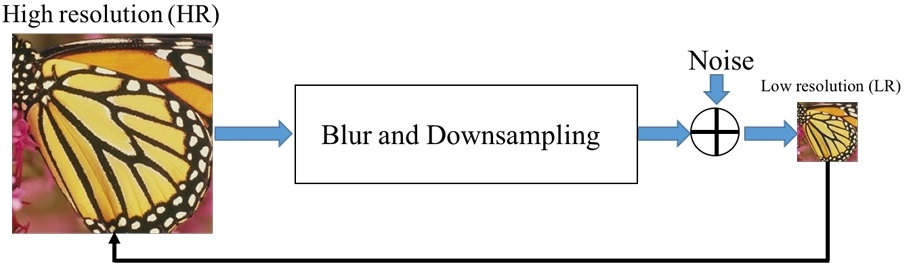
\includegraphics[totalheight=1.5in]{Chapter1/Fig6.jpg}
    \caption[Recovering HR from its LR components]{Recovering HR from its LR components.\cite{DLSR}}
    \label{fig:label1.3}
\end{figure}
Interpolation-based SISR approaches, such as bicubic interpolation\cite{Bicubic} and Lanczos resampling \cite{lanczos}, are relatively quick and simple although they lack precision. Reconstruction-based SR approaches that frequently employ sophisticated previous information to restrict the available solution space, with the benefit of producing flexible and sharp details. Nevertheless, the performance of many reconstruction-based methods rapidly decreases as the scale factor grows, and these techniques are typically time-consuming.
\newpage
\section{Motivation}
The visual interpretation and automated analysis of endoscopic recordings are hampered by artefacts such as motion blur, bubbles, specular reflections, floating objects, and pixel saturation. Given the increasing use of endoscopy in many clinical applications, a key medical imaging challenge is identifying such artefacts and automating the repair of damaged video frames. The doctor is likely to miss a key frame that reveals the irregularity because the video is the same length as the time it takes for the capsule to pass through the intestines. To address the prevailing procedures, Computer-Aided Detection (CAD) approaches were proposed.
The use of computers to detect abnormalities in capsule endoscopy images has opened up new research opportunities in the fields of medical image processing and machine learning and deep learning. Deep learning has been proven to be one of the most efficient method to deal with images, whether it be image classification, image segmentation or object detection in images.
The accuracy of these algorithms highly depend on the resolution of the images. Also, it is very easy for the doctors to detect the abnormalities with naked eye. Hence, We decided to work on this problem statement. 
\section{Objective}
Wireless Capsule Endoscopy is gaining vast acceptance in society, and there is a severe need of computer aided tools to process the data obtained from the images. Our main objective is to increase the resolution of these images by a factor of 4, so that the images have better perceptual quality and the higher resolution of these images can be used to improve the accuracy of the computer aided algorithms.
\section{Report outline}
The report is organized such that Chapter 2 shows the extensive literature review which covers traditional up-sampling methods such as bi-cubic interpolation, nearest neighbour interpolation, etc. as well as deep learning based up-sampling methods, Chapter 3 describes state of the art models for image super resolution and their performance on wireless capsule dataset, while Chapter 4 demonstrates the proposed architecture and their training details.
Chapter 5 shows the comparative study of results obtained during experimental work and the report ends with summary and future scope.



